\documentclass{article}
\usepackage[utf8]{inputenc}
\usepackage[T1]{fontenc}
\usepackage{geometry}
\usepackage{enumitem}
\usepackage{graphicx}

\geometry{margin=0.5in}

\begin{document}

\title{\textbf{Konwerter analog-cyfra \textit{(ADC)}}
\\ \large{Bazując na wiedzy \textit{dr. inż. Macieja Dzieniakowskiego}}}
\author{\textbf{Adrian Chmiel}}
\date{23 maja 2024}
\maketitle

\section{Cel zadania}
Sygnał nadawany przez konwerter ADC sterowany przez przełącznik A1 podawany \textit{(z opóźnieniem)} do konwerterów DAC i wyświetlany na ekranie oscyloskopu.

\section{Konfiguracja}
Konfiguracja dzieli się na trzy zasadnicze kroki:
\begin{enumerate}[label=\arabic*.]
    \item \textbf{Konfiguracja konwerterów DAC}
    \item \textbf{Konfiguracja konwertera ADC}
    \item \textbf{Ustawienie przełącznika A1 jako kanał wejściowy}
\end{enumerate}
Taki też podział znajduje się w dalszej części dokumentu i zalecane jest zachowanie tej kolejności w celu minimalizacji napotkanych problemów.

\section{Inne uwagi}
Najpierw otrzymaliśmy parę rad, które warto zawrzeć na początku:
\begin{itemize}
    \item Prawidłowa konfiguracja konwertera ADC nie jest prostym zadaniem, szczególnie jak robimy to po raz pierwszy
    \item Dostępna konfiguracja konwertera ADC pozwala na sporą kontrolę nad sygnałem poprzez wiele dostępnych parametrów
    \item Domyślne wartości bitów przy każdym parametrze to \textbf{0}, co oznacza, że nie musimy ich zawsze ustawiać
\end{itemize}
Zalecane jest postępowanie według poniższego schematu:
\vspace{3mm} \\
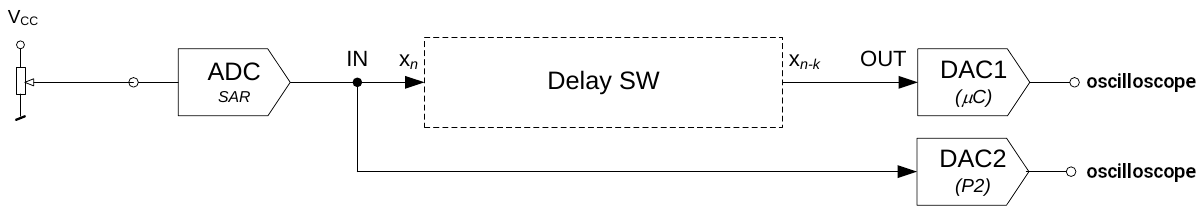
\includegraphics[width=\textwidth]{"../adc_img/ADC_delay_DAC_1.png"}
\textit{Źródło: ADC\_delay\_DAC.pdf, strona: 1}
\vspace{3mm} \\
\textbf{\textit{Delay SW}} oznacza oprogramowanie (w tym przypadku fragment kodu) opóźniające sygnał.
Wykreśliłem ten element za pomocą przerywanej linii tak, aby oznaczyć, że jak na razie nie jest on dla nas istotny.
Nie oznacza to jednak, że to oprogramowanie nie powinno się tam znaleźć w finalnej wersji programu.

\section{Konfiguracja konwerterów DAC}
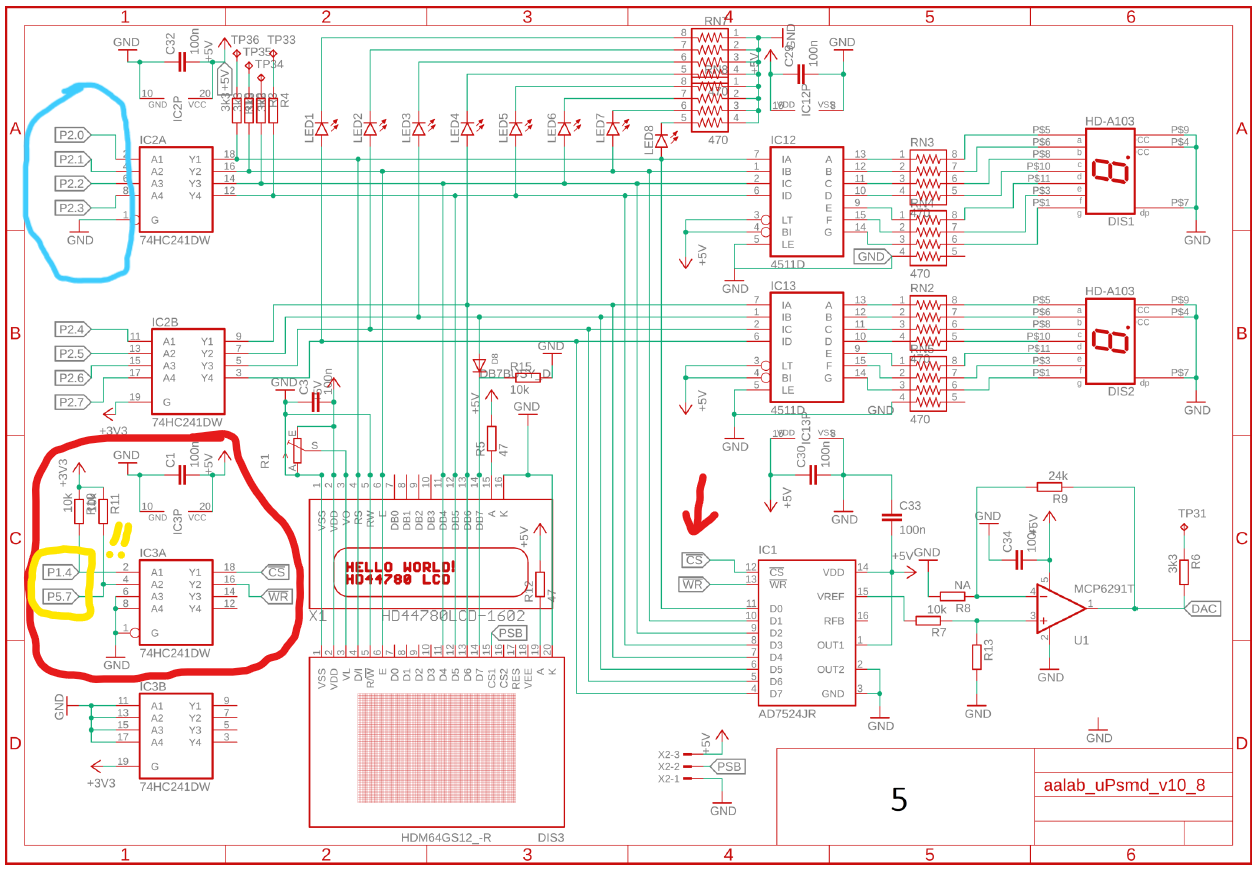
\includegraphics[width=\textwidth]{"../adc_img/Schemat_bloki_7.png"}
\textit{Źródło: Schemat\_bloki.pdf, strona: 7}
\vspace{3mm} \\
Zgodnie z widocznym powyżej schematem konieczna jest konfiguracja portów \textit{P1.4} oraz \textit{P5.7} jako \textbf{wyjściowych} tak, aby możliwe było oglądanie rezultatów na ekranie oscyloskopu po podpięciu go do odpowiednich pinów.
Oprócz tego konieczne jest ustawienie wszystkich pinów z portu \textit{P2} jako \textbf{wyjściowe}.
Dokonać tego możemy następującym fragmentem kodu w sekcji inicjalizacji:
\begin{verbatim}
BIS.B #00010000b, &P1DIR ; set P1.4 as out
BIS.B #10000000b, &P5DIR ; set P5.7 as out
BIC.B #00010000b, &P1OUT ; clear bit P1.4
BIC.B #10000000b, &P5OUT ; clear bit P5.7
MOV.B #255, P2DIR        ; set all pins from port 2 as outputs
MOV.B #0, P2OUT          ; set port 2 to low \end{verbatim}
\newpage
Resztę konfiguracji możemy dokonać za pomocą kodu, który wcześniej otrzymaliśmy podczas \textbf{zadania z timerem}:
\begin{verbatim}
     ;---------- Basic Clock Module Initialisation --------------------------------------
     ; - switch from DCO to XT2
     ; - MCLK & SMCLK supplied from XT2, ACLK = n/a
     ; - the DCO is left runing
     bis.b #OSCOFF,SR ;turn OFF osc.1
     bic.b #XT2OFF,BCSCTL1 ;turn ON osc.2
BCM0 bic.b #OFIFG,&IFG1 ;clear OFIFG
     mov #0FFFFh,R15 ;delay (waiting for oscilator start)
BCM1 dec R15 ;delay
     ;jnz BCM1 ;delay -> commented out as it was ocasionally leading to infinite loop
     bit.b #OFIFG,&IFG1 ;test OFIFG
     jnz BCM0 ;repeat test if needed
     ;MCLK
     bic.b #040h,&BCSCTL2 ;slelect XT2CLK as source
     bis.b #080h,&BCSCTL2 ;
     bic.b #030h,&BCSCTL2 ;MCLK=source/1 (8MHz)
     ;SMCLK
     bis.b #SELS,&BCSCTL2 ;slelect XT2CLK as source
     bic.b #006h,&BCSCTL2 ;SMCLK=source/1 (8MHz)
     ;---

     ;... ;DAC_0 initialisation 
     bis.w #REFON+REF2_5V,&ADC12CTL0 ;Reference generator ON, VRef+=2.5V
     bic #DAC12SREF0,&DAC12_0CTL ;set Vref=VREF+
     bic #DAC12SREF1,&DAC12_0CTL ;
     bic #DAC12RES,&DAC12_0CTL ;12-bit resolution
     bic #DAC12LSEL0,&DAC12_0CTL ;Load mode 0
     bic #DAC12LSEL1,&DAC12_0CTL ;
     bis #DAC12IR,&DAC12_0CTL ;Full-Scale=1xVref
     bis #DAC12AMP0,&DAC12_0CTL ;High speed amplifier output 
     bis #DAC12AMP1,&DAC12_0CTL ; 
     bis #DAC12AMP2,&DAC12_0CTL ;
     bic #DAC12DF,&DAC12_0CTL ;Data format - straight binary 
     bic #DAC12IE,&DAC12_0CTL ;Interrupt disabled 
     bis #DAC12ENC,&DAC12_0CTL ;DAC_0 conversion enabled 
     ;...

     ;... ;DAC_1 initialisation 
     bis.w #REFON+REF2_5V,&ADC12CTL0 ;Reference generator ON, VRef+=2.5V
     bic #DAC12SREF0,&DAC12_1CTL ;set Vref=VREF+
     bic #DAC12SREF1,&DAC12_1CTL ;
     bic #DAC12RES,&DAC12_1CTL ;12-bit resolution
     bic #DAC12LSEL0,&DAC12_1CTL ;Load mode 0
     bic #DAC12LSEL1,&DAC12_1CTL ;
     bis #DAC12IR,&DAC12_1CTL ;Full-Scale=1xVref
     bis #DAC12AMP0,&DAC12_1CTL ;High speed amplifier output 
     bis #DAC12AMP1,&DAC12_1CTL ; 
     bis #DAC12AMP2,&DAC12_1CTL ;
     bic #DAC12DF,&DAC12_1CTL ;Data format - straight binary 
     bic #DAC12IE,&DAC12_1CTL ;Interrupt disabled 
     bis #DAC12ENC,&DAC12_1CTL ;DAC_1 conversion enabled 
     ;... \end{verbatim}
\section{Konfiguracja konwerterów ADC}
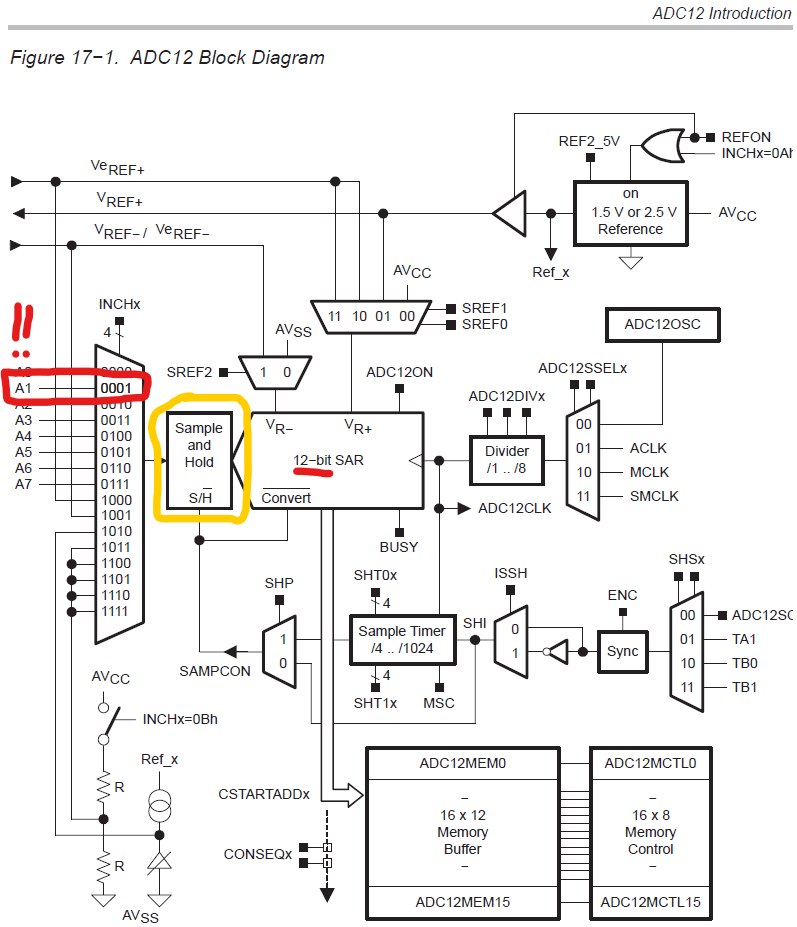
\includegraphics[width=\textwidth]{"../adc_img/slau049f_346.png"} \\
\textit{Źródło: slau049f.pdf, strona: 346}
\newpage
Konfiguracja konwertera ADC jest nieco bardziej skomplikowana niż konfiguracja konwerterów DAC. Warto zwrócić uwagę na parę aspektów:
\begin{itemize}
    \item Przetwornik ADC jest \textbf{12-bitowy}, lecz w rzeczywistości będzie nas interesować jedynie \textbf{8 młodszych bitów}, ponieważ jeden używanych przetworników DAC jest tylko 8-bitowy.
    \item Parametr \textit{Sample and Hold} pozwala na pobranie próbki i jej przetrzymanie - jest to konieczne do prawidłowego działania konwertera z opóźnieniem.
\end{itemize}
Cały proces konfiguracji możemy podzielić na trzy kroki:
\begin{enumerate}[label=\arabic*.]
    \item \textbf{Wstępna konfiguracja ADC12CTL0}
\vspace{3mm} \\
Dokumentacja odpowiadająca temu krokowi znajduje się poniżej: \\
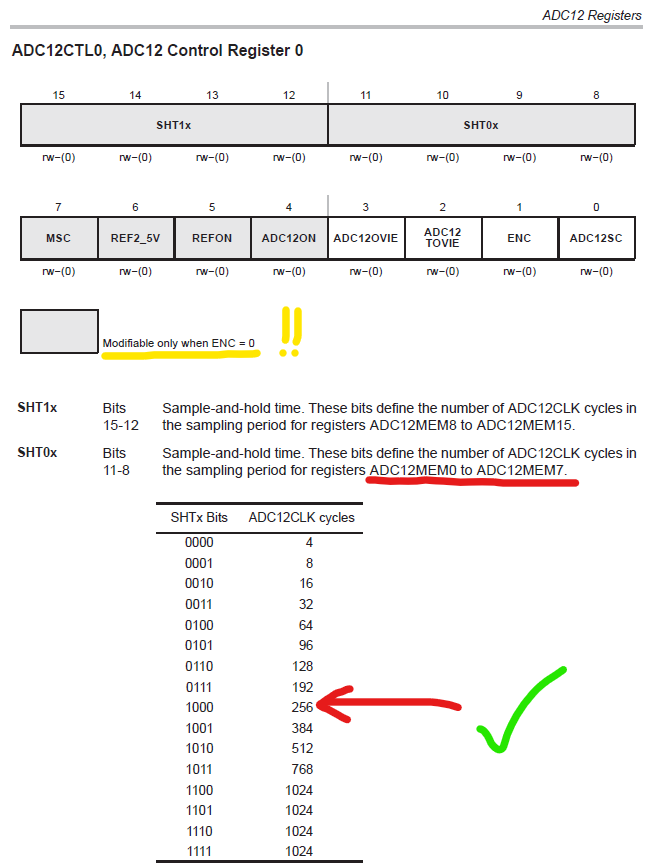
\includegraphics[width=0.775\textwidth]{"../adc_img/slau049f_364.png"} \\
\textit{Źródło: slau049f.pdf, strona: 364}
\vspace{3mm} \\
Ze względu na to, że będziemy zajmować się jedynie liczbami 8-bitowymi wystarczą nam komórki \textit{ADC12MEM0 - ADC12MEM7}.
Z tego powodu wystarczy, że ustawimy jedynie czas przetrzymywania próbki \textit{SHT0} odpowiadający tym komórkom. Zalecany czas to \textbf{256 cyklów} zegara! \\
\vspace{3mm} \\
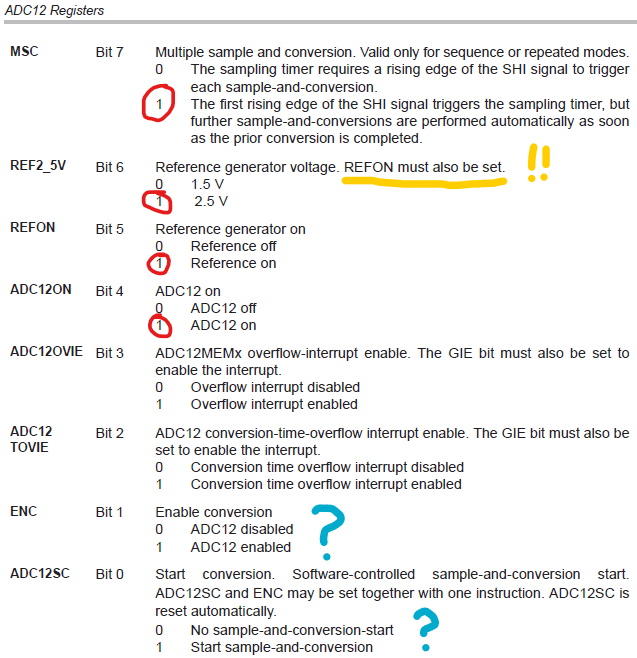
\includegraphics[width=0.875\textwidth]{"../adc_img/slau049f_365.png"} \\
\textit{Źródło: slau049f.pdf, strona: 365}
\vspace{3mm} \\
Ta część wymaga dokładnego zrozumienia powyższego fragmentu dokumentacji, gdyż zmieniamy tutaj dość dużo parametrów.
\begin{itemize}
     \item \textit{MSC} - pozwala na to, aby następne konwersje wykonywały się automatycznie jedna po drugiej
     \item \textit{REF2\_5V} - ustawiamy napięcie referencyjne na 2.5V
     \item \textit{REFON} - włączamy generator napięcia referencyjnego
     \item \textit{ADC12ON} - włączamy konwerter ADC
     \item \textit{ADC12OVIE \& ADC12TOVIE} - odpowiadają za przerwanie, z którego nie będziemy korzystać, a więc wartość bitu zostaje bez zmian
     \item \textit{ENC} - pozwala na konwersję \textbf{(ustawiane dopiero na końcu całej konfiguracji!)}
     \item \textit{ADC12SC} - rozpoczęcie konwersji \textbf{(ustawiane dopiero na końcu całej konfiguracji!)}
\end{itemize}
Kod wykonujący ten krok znajduje się poniżej:
\begin{verbatim}
BIS.W #0000100011110000b, &ADC12CTL0
; SHT0 = 1000b (256 cycles) | MSC = 1 | REF2_5V = 1 | REFON = 1 | ADC12ON = 1 \end{verbatim}
    \item \textbf{Konfiguracja ADC12CTL1}
    \vspace{3mm} \\
Dokumentacja odpowiadająca temu krokowi znajduje się poniżej: \\
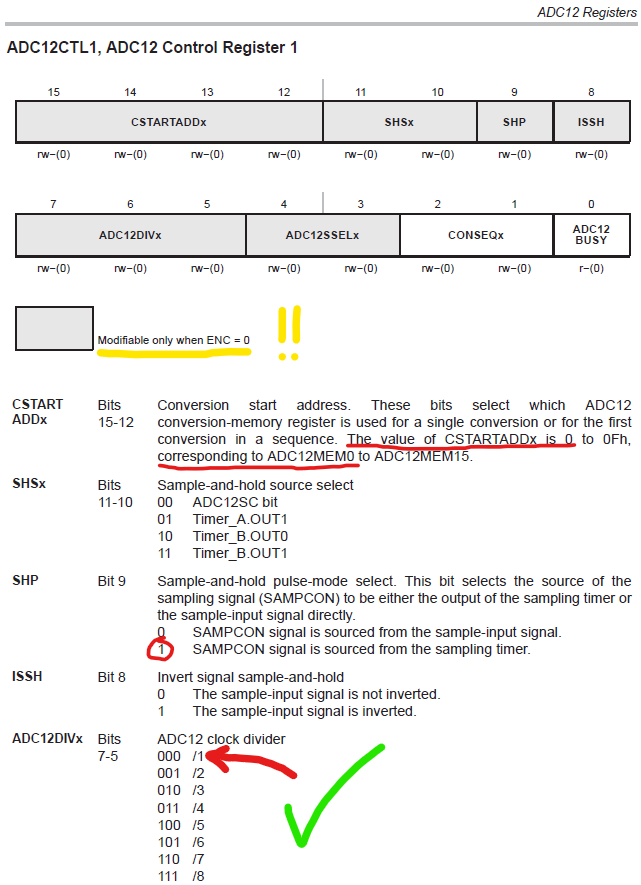
\includegraphics[width=0.825\textwidth]{"../adc_img/slau049f_366.png"} \\
\textit{Źródło: slau049f.pdf, strona: 366}
\vspace{3mm} \\
W tym kroku istotne są następujące parametry:
\begin{itemize}
     \item \textit{CSTARTADDx} - w tym adresie zacznie się zapis wyniku konwersji - zostawiamy bez zmian, a więc będzie to \textit{ADC12MEM0}
     \item \textit{SHP} - pozwala na to, aby sygnał zewnętrzny sterował konwersją (tj. w naszym wypadku \textbf{przełącznik A1})
     \item \textit{ADC12DIVx} - ta wartość dzieli zegar, którym pracuje konwerter - zostawiamy bez zmian, aby nie zmieniać częstotliwości zegara, lecz warto zwrócić uwagę, że jest to parametr, który można potem zmieniać w zależności od potrzeb
\end{itemize}
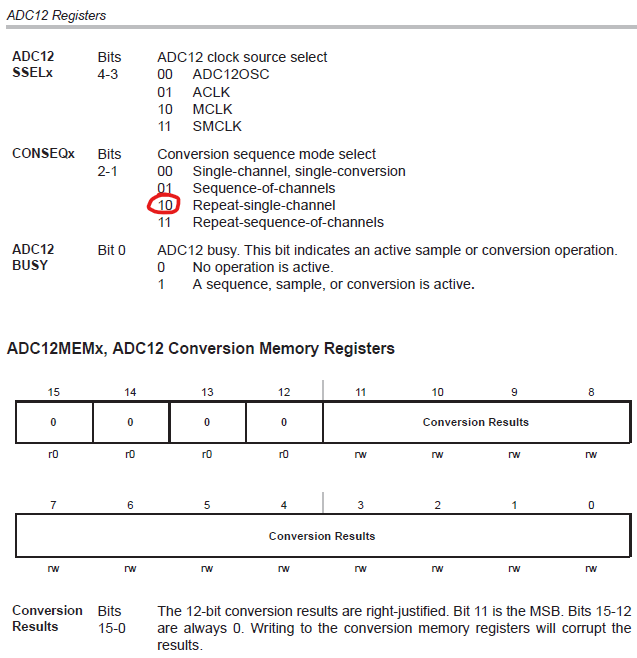
\includegraphics[width=0.9\textwidth]{"../adc_img/slau049f_367.png"} \\
\textit{Źródło: slau049f.pdf, strona: 367}
\vspace{3mm} \\
Zmieniamy parametr \textit{CONSEQx} na \textbf{10}, aby konwersja cały czas była \textbf{powtarzana} bazując na \textbf{pojedynczym} kanale z przetwornikiem A1.
Kod wykonujący cały krok z konfiguracją \textit{ADC12CTL1} znajduje się poniżej:
\begin{verbatim}
BIS.W #0000001000000010b, &ADC12CTL1
; SHP = 1 | CONSEQ2 = 1 -> A1 goes to MEM0 \end{verbatim}
\newpage
    \item \textbf{Konfiguracja ADC12MCTL0}
     \vspace{3mm} \\
Dokumentacja odpowiadająca temu krokowi znajduje się poniżej: \\
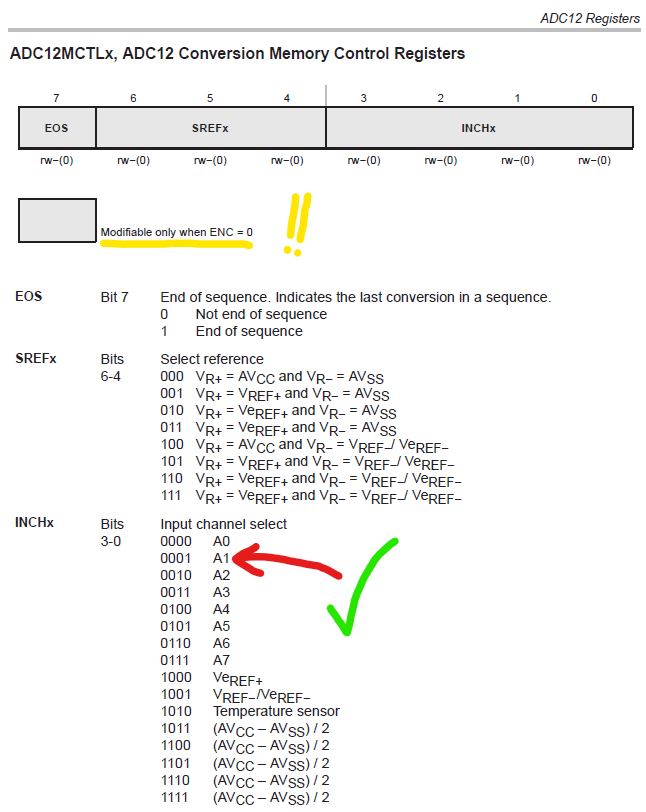
\includegraphics[width=0.9\textwidth]{"../adc_img/slau049f_368.png"} \\
\textit{Źródło: slau049f.pdf, strona: 368}
\vspace{3mm} \\
Jedyne co wykonujemy w tym kroku, to ustawienie kanału wejściowego na \textbf{A1}, co umożliwi prawidłowe działanie przełącznika.
Osiągamy to przez ustawienie rejestru \textit{INCHx} na wartość \textbf{0001}. Kod wykonujący tą konfigurację znajduje się poniżej:
\begin{verbatim}
BIS.B #00000001b, &ADC12MCTL0 ; set input channel as A1 \end{verbatim}
     \item \textbf{Dozwolenie na konwersję oraz jej wystartowanie}
     \vspace{3mm} \\
Ponownie wracamy do konfiguracji \textit{ADC12CTL0}. Ten krok koniecznie musi zostać wykonany jako ostatni element konfiguracji, gdyż uniemożliwia on zmianę większości z pozostałych ustawień zmodyfikowanych wcześniej.
W tym celu zmieniamy wartości rejestrów \textit{ENC} oraz \textit{ADC12SC} na wartość \textbf{1}.
\vspace{3mm} \\
Kod wykonujący ten krok znajduje się poniżej:
\begin{verbatim}
BIS.W #11b, &ADC12CTL0 ; has to be at the end
; ENC = 1 | ADC12SC = 1 -> enables and starts conversion \end{verbatim}
\end{enumerate}

\section{Ustawienie przełącznika A1 jako kanał wejściowy}
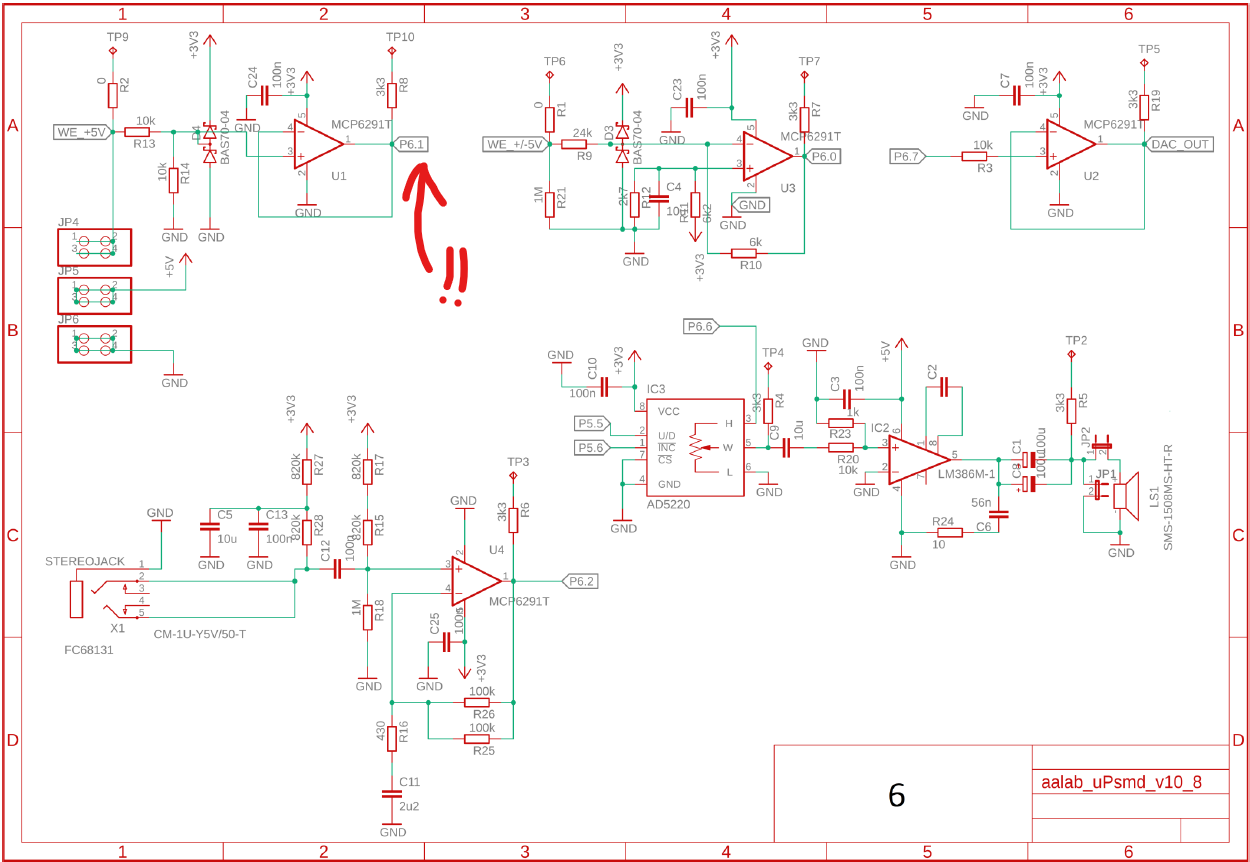
\includegraphics[width=\textwidth]{"../adc_img/Schemat_bloki_8.png"}
\textit{Źródło: Schemat\_bloki.pdf, strona: 8}
Częściowo wykonaliśmy już to zadanie w krokach poprzednich, lecz identycznie jak w przypadku konwerterów powyżej, konieczne jest ustawienie pewnych bitów na konkretne wartości.
W tym przypadku konieczne jest ustawienie portu \textit{P6.1} jako \textbf{wejście analogowe} rejestrem \textit{P6SEL} przy użyciu następującego kodu:
\begin{verbatim}
BIS.B #10b, &P6SEL ; set P6.1 as analog input \end{verbatim}
Fakt ten możemy poprzeć fragmentem dokumentacji, który znajduje się poniżej: \\
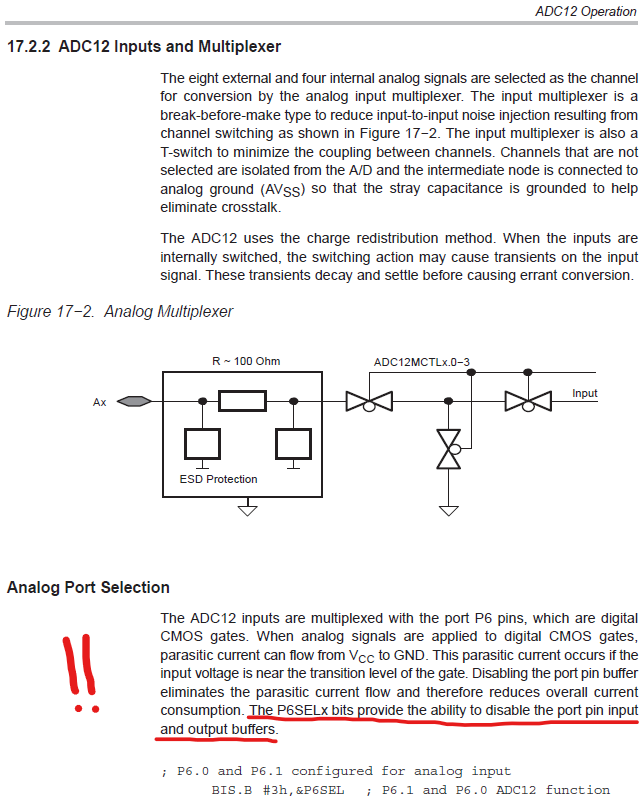
\includegraphics[width=0.9\textwidth]{"../adc_img/slau049f_348.png"} \\
\textit{Źródło: slau049f.pdf, strona: 348}

\section{Kompletny kod z konfiguracją}
Kompletny kod programu z konfiguracją widoczny jest poniżej \textbf{(może zawierać błędy)}.
\newpage
\begin{verbatim}
#include "msp430.h"                  ; #define controlled include file
 
     NAME    main                    ; module name

     PUBLIC  main                    ; make the main label vissible
                                     ; outside this module
     ORG     0FFECh
     DC16    TIMER_A0_Interrupt
     ORG     0FFFEh                  
     DC16    init                    ; set reset vector to 'init' label

     RSEG    CSTACK                  ; pre-declaration of segment
     RSEG    CODE                    ; place program in 'CODE' segment

init:   MOV     #SFE(CSTACK), SP        ; set up stack
     ; DAC_2 (P2) config
     BIS.B #00010000b, &P1DIR ; set P1.4 as out
     BIS.B #10000000b, &P5DIR ; set P5.7 as out
     BIC.B #00010000b, &P1OUT ; clear bit P1.4
     BIC.B #10000000b, &P5OUT ; clear bit P5.7
     MOV.B #255, P2DIR        ; set all pins from port 2 as outputs
     MOV.B #0, P2OUT          ; set port 2 to low

     ; ADC config (based on documentation)
     BIS.W #0000100011110000b, &ADC12CTL0
     ; SHT0 = 1000b (256 cycles) | MSC = 1 | REF2_5V = 1 | REFON = 1 | ADC12ON = 1
     BIS.W #0000001000000010b, &ADC12CTL1
     ; SHP = 1 | CONSEQ2 = 1 -> A1 forwarded to MEM0
     BIS.B #00000001b, &ADC12MCTL0 ; set input channel as A1
     BIS.B #10b, &P6SEL ; set P6.1 as analog input
     BIS.W #11b, &ADC12CTL0 ; has to be at the end
     ; ENC = 1 | ADC12SC = 1 -> enables and starts conversion

     ;---------- Basic Clock Module Initialisation --------------------------------------
     ; - switch from DCO to XT2
     ; - MCLK & SMCLK supplied from XT2, ACLK = n/a
     ; - the DCO is left runing
     bis.b #OSCOFF,SR ;turn OFF osc.1
     bic.b #XT2OFF,BCSCTL1 ;turn ON osc.2
BCM0 bic.b #OFIFG,&IFG1 ;clear OFIFG
     mov #0FFFFh,R15 ;delay (waiting for oscilator start)
BCM1 dec R15 ;delay
     ;jnz BCM1 ;delay -> commented out as it was ocasionally leading to infinite loop
     bit.b #OFIFG,&IFG1 ;test OFIFG
     jnz BCM0 ;repeat test if needed
     ;MCLK
     bic.b #040h,&BCSCTL2 ;slelect XT2CLK as source
     bis.b #080h,&BCSCTL2 ;
     bic.b #030h,&BCSCTL2 ;MCLK=source/1 (8MHz)
     ;SMCLK
     bis.b #SELS,&BCSCTL2 ;slelect XT2CLK as source
     bic.b #006h,&BCSCTL2 ;SMCLK=source/1 (8MHz)
     ;---

     ;... ;DAC_0 initialisation 
     bis.w #REFON+REF2_5V,&ADC12CTL0 ;Reference generator ON, VRef+=2.5V
     bic #DAC12SREF0,&DAC12_0CTL ;set Vref=VREF+
     bic #DAC12SREF1,&DAC12_0CTL ;
     bic #DAC12RES,&DAC12_0CTL ;12-bit resolution
     bic #DAC12LSEL0,&DAC12_0CTL ;Load mode 0
     bic #DAC12LSEL1,&DAC12_0CTL ;
     bis #DAC12IR,&DAC12_0CTL ;Full-Scale=1xVref
     bis #DAC12AMP0,&DAC12_0CTL ;High speed amplifier output 
     bis #DAC12AMP1,&DAC12_0CTL ; 
     bis #DAC12AMP2,&DAC12_0CTL ;
     bic #DAC12DF,&DAC12_0CTL ;Data format - straight binary 
     bic #DAC12IE,&DAC12_0CTL ;Interrupt disabled 
     bis #DAC12ENC,&DAC12_0CTL ;DAC_0 conversion enabled 
     ;...

     ;... ;DAC_1 initialisation 
     bis.w #REFON+REF2_5V,&ADC12CTL0 ;Reference generator ON, VRef+=2.5V
     bic #DAC12SREF0,&DAC12_1CTL ;set Vref=VREF+
     bic #DAC12SREF1,&DAC12_1CTL ;
     bic #DAC12RES,&DAC12_1CTL ;12-bit resolution
     bic #DAC12LSEL0,&DAC12_1CTL ;Load mode 0
     bic #DAC12LSEL1,&DAC12_1CTL ;
     bis #DAC12IR,&DAC12_1CTL ;Full-Scale=1xVref
     bis #DAC12AMP0,&DAC12_1CTL ;High speed amplifier output 
     bis #DAC12AMP1,&DAC12_1CTL ; 
     bis #DAC12AMP2,&DAC12_1CTL ;
     bic #DAC12DF,&DAC12_1CTL ;Data format - straight binary 
     bic #DAC12IE,&DAC12_1CTL ;Interrupt disabled 
     bis #DAC12ENC,&DAC12_1CTL ;DAC_1 conversion enabled 
     ;... 

main:   NOP                             ; main program
     MOV.W   #WDTPW+WDTHOLD,&WDTCTL  ; Stop watchdog timer
     mov.w   #0x5,&TACCR0            ; Period for up mode
     mov.w   #CCIE,&TACCTL0          ; Enable interrupts on Compare 0
     mov.w   #MC_1|ID_3|TASSEL_2|TACLR,&TACTL
     bis.w   #GIE,SR                 ; Enable interrupts (just TACCR0)

Mainloop:
     nop                             ; Required only for debugger
     JMP $                           ; jump to current location '$'                                       
                                     ; (endless loop)

TIMER_A0_Interrupt:
     MOV.W  &ADC12MEM0, R5           ; moving the value from ADC to R5
     MOV    R5, &DAC12_1DAT          ; moving that value to converter DAC_1 
     MOV.B  R5, &P2OUT               ; moving that value to converter DAC_2
     RETI

     END\end{verbatim}
\end{document}